%% Elsevier LaTeX Template for Remote Sensing of Environment
\documentclass[preprint,12pt,authoryear]{elsarticle}
% 1. Load lineno (BEFORE hyperref if you use it)
\usepackage{lineno}

\usepackage{wrapfig}
\setlength{\intextsep}{10pt}   % space above/below wrapped figures
\setlength{\columnsep}{20pt}   % space between figure and text
\usepackage{booktabs}
\usepackage{placeins}
\usepackage{float}
% Placeholder for figure paths
% \newcommand{\manuscriptfigurepath}{manuscript/figures/} % If your path is different
\usepackage{tabularx}
%% Package imports
\usepackage{amssymb}
\usepackage{amsmath}
\usepackage{xcolor} % For \textcolor
\usepackage[margin=1in]{geometry}
\usepackage{enumitem}
\bibliographystyle{elsarticle-harv}
\usepackage{graphicx}
\graphicspath{{manuscript/figures/}}
\usepackage{lineno} %% Uncomment for line numbering
\usepackage{siunitx} 
\usepackage{caption}

\setlist[itemize,1]{leftmargin=*}

% \linenumbers
% \modulolinenumbers[2]
%% Journal name
% \journal{Remote Sensing of Environment}

\begin{document}

\begin{frontmatter}

%% Title, author info
\title{Attention-Based Upsampling of Airborne LiDAR in Natural Landscapes with SAR and Optical Imagery Fusion}


\author[affil]{Michael Marks}
\cortext[cor1]{Corresponding author} 
\ead{mmarks13@gmail.com}

\affiliation[affil]{organization={Department of Geography, San Diego State University},
            state={California},
            country={United States}}

%% Abstract
\begin{abstract}
Accurate and timely 3D vegetation structure information is essential for ecological modeling and land management; however, meeting this need often encounters obstacles with national airborne LiDAR surveys, whose broad-area coverage comes with trade-offs in point density and update frequency.  This study introduces an attention-based deep learning framework to upsample sparse airborne LiDAR point clouds by fusing them with current high-resolution optical (NAIP) and L-band Synthetic Aperture Radar (UAVSAR) imagery. Utilizing a novel Local-Global Point Attention Block (LG-PAB), our model directly enhances 3D point cloud density and accuracy in natural landscapes. Results demonstrate that fusing both optical and radar imagery significantly reduces reconstruction error (Chamfer distance) compared to using LiDAR alone or with a single image modality. Notably, the fused model substantially mitigates errors arising from vegetation changes over time, particularly in areas of canopy loss, thereby increasing the utility of historical LiDAR archives. This research presents a novel approach for direct 3D point cloud enhancement, moving beyond traditional raster-based methods and offering a pathway to more accurate and timely vegetation structure assessments.
\end{abstract}

% %% Research highlights
% \begin{highlights}
% \item Key finding or contribution 1
% \item Key finding or contribution 2
% \end{highlights}

% %% Keywords
% \begin{keyword}
% Keyword 1 \sep Keyword 2 \sep Keyword 3
% \end{keyword}

\end{frontmatter}


%% Main manuscript body


\section{Introduction}

Accurate three-dimensional (3D) vegetation structure information at submeter spatial scales is increasingly essential for applications ranging from wildfire risk modeling \citep{martin-ducup_unlocking_2025} to biodiversity and habitat assessment \citep{Merrick2013Into3D,moudry2023vegetation}. The way vegetation is arranged—its height, density, and continuity—directly influences both fire hazard and fire behavior, and impacts how species use the landscape. Fuels, as opposed to topography and weather, are the only element of the fire behavior triangle that land managers can directly manipulate \citep{agee_influence_1996}, making structural data vital for strategic interventions. Simultaneously, vegetation structure governs microclimate, resource availability, and landscape connectivity, making it a cornerstone of ecological monitoring and conservation planning \citep{guo2018integrating, mahata2023microclimate,ustin2021current}. Airborne light detection and ranging (LiDAR) has emerged as a premier tool for capturing this structural complexity, enabling detailed, landscape-scale mapping of vegetation structure that was previously unattainable with passive optical imagery \citep{Merrick2013Into3D, belov2019capabilities, guo2020lidar}. 

National mapping programs such as the U.S. Geological Survey's 3D Elevation Program (3DEP) now collect LiDAR data over large areas, but these surveys have important limitations. Typical 3DEP acquisitions are performed at modest point densities (on the order of \qtyrange{0.5}{20}{pts\per\square\meter}) \citep{wu2016evaluating} and with much of the national LiDAR baseline acquired over an extended period (e.g., roughly 2015-2023), a significant portion of this foundational data is now several years old, a situation exacerbated by the lack of a guaranteed or universal update timeline \citep{usgs_what_2019}. Consequently, the available point clouds often reflect conditions from several years prior and are relatively sparse compared to those obtained from other platforms (e.g. UAV, see figure \ref{fig:als_v_uav}).
\begin{figure}[!b]
    \centering
    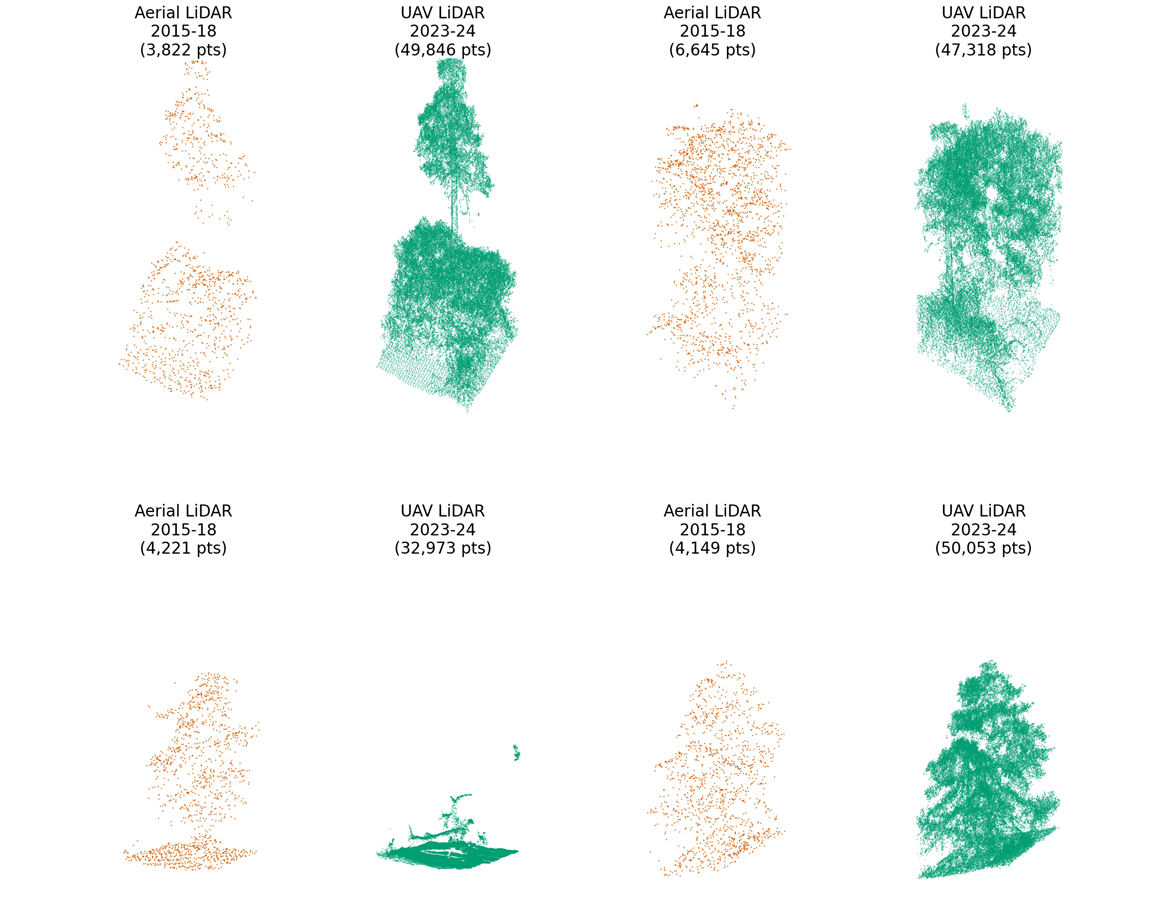
\includegraphics[trim={15mm 5mm 15mm 0mm},width=1\linewidth]{manuscript//figures/als_vs_uavls.png}
    \caption{Comparison of \SI{100}{\square\meter} point clouds from USGS 3DEP aerial LiDAR (2015--2018, orange) and UAV LiDAR (2023--2024, green) over the same locations. UAV LiDAR captures significantly greater structural detail, especially in fine-scale canopy features. The bottom-left example shows clear canopy loss between surveys due to recent disturbance.}
    \label{fig:als_v_uav}
\end{figure}
Critical changes in vegetation structure, such as disturbance-driven loss or ongoing vegetation growth, may go undetected between LiDAR acquisition cycles. This sparsity and temporal gap limit the utility of national LiDAR datasets for applications that require up-to-date, high-resolution 3D information.

Given the limitations of national LiDAR in spatial and temporal resolution, one promising avenue is to enrich these sparse datasets using co-registered imagery from other remote sensing platforms that offer more frequent updates. High-resolution aerial imagery—such as orthophotos from the National Agriculture Imagery Program (NAIP) \citep{usda_naip_2024}—provides fine detail on canopy textures, gaps, and vegetation color, typically acquired at 2 year intervals. Complementing this, L-band synthetic aperture radar known for its sensitivity to vegetation structure \citep{wang2025interpretable}, can provide valuable multi-temporal data through repeat acquisitions. NASA’s UAVSAR \citep{rosen2006uavsar}, for example, conducts bi-annual L-band campaigns to monitor San Andreas fault movement, and the upcoming NISAR satellite mission will offer global L-band SAR at a 12-day revisit rate \citep{kellogg2020nasa}. Fusing such temporally rich optical and radar imagery with existing LiDAR has the potential to produce a denser 3D point cloud reflecting more current vegetation conditions—a challenge well-suited to data-driven approaches such as deep learning. In particular, attention-based models offer a powerful way to integrate these diverse inputs by modeling their spatial and semantic relationships.



Attention mechanisms, first introduced for language translation by \citep{bahdanau2014neural}, enable a model to dynamically determine which parts of input data are most relevant to each other, a capability crucial for understanding complex scenes. For example, in point clouds of natural landscapes, a point on a tree’s leaf can learn, through self-attention, to connect more strongly with its own trunk or branches than with foliage from an adjacent, albeit closer, tree. This ability to discern intrinsic structural relationships could be particularly effective in natural vegetation, as its fractal and self-similar nature provides consistent patterns for self-attention to model across different scales \citep{scheuring1994application, yang2015extraction}. When fusing data, cross-attention extends this by allowing features from one modality, such as a LiDAR point, to selectively query information from another modality, like relevant shadow patterns or canopy gaps identified in NAIP imagery or radar data. These powerful attention operations are the fundamental building block of the influential Transformer architecture \citep{vaswani2017attention}, which serves as the foundation for nearly all large language model architectures in use today. Building on that success, Transformers were adapted for vision tasks \citep{dosovitskiy2020image} and are now increasingly used across many remote sensing tasks \citep{aleissaee2023transformers}. While these advancements showcase their broad utility, their specific application and optimal adaptation for enhancing sparse airborne LiDAR in complex natural landscapes present unique challenges and open questions.

Consequently, key knowledge gaps remain. First, most prior work on data-driven LiDAR enhancement has focused on enhancing point-cloud-derived metrics in raster form (e.g. canopy height \citep{wilkes_mapping_2015, wagner_sub-meter_2024}, above-ground biomass \citep{shendryk2022fusing}, elevation \citep{li2023large}, and other fuel/vegetation metrics \citep{taneja2023up, gazzea2023high}) rather than directly enhancing the point cloud itself. Although one recent study successfully upsampled mobile laser scanner point clouds in a forested environment using terrestrial LiDAR as ground truth \citep{remijnse2024upsampling}, both sensors differ substantially from airborne systems in scale and occlusion behavior. Second, existing deep learning frameworks for point cloud upsampling have primarily been developed and tested on synthetic shapes or man-made objects, and their efficacy on the complex, irregular structures of natural vegetation is not well understood. Third, our extensive literature review found no studies that have attempted to leverage optical or radar imagery for enhancing point clouds in natural landscapes. Third, our review also found no studies that have analyzed model performance when the LiDAR input is temporally misaligned with the ground truth due to vegetation dynamics. Deep models are typically trained and evaluated on static scenes, often using an artificially down-sampled high-density point cloud as the input. Thus, it remains unknown how upsampling errors behave in areas where substantial canopy growth or loss has occurred since the original LiDAR survey, or whether multi-modal inputs can mitigate errors stemming from such changes.

\subsection{Background and Related Work}

\subsubsection{Point Cloud Upsampling with Deep Learning}

In computer vision and graphics, a range of neural frameworks have been proposed to densify sparse point clouds. PU-Net \citep{yu2018pu} pioneered the task with multi-scale multi-layer perceptron (MLP) feature extraction and a point-set expansion module, achieving good fidelity on synthetic computer-designed (CAD) objects. PU-GCN (Point Upsampling-Graph Convolution Network) later built upon this by replacing the expansion MLP with a graph-convolution upsampling unit called \emph{NodeShuffle} and paired it with a GCN feature extractor \citep{qian2021pu}. Recently, PU-Transformer introduced the first transformer-based upsampler to exploit both local and long-range relations \citep{qiu2022pu}. While these methods deliver state-of-the-art results on synthetic shapes and man-made objects, their behavior on the irregular geometry of natural vegetation—and in LiDAR-derived point clouds more broadly—remains largely untested.


\subsubsection{Upsampling in Natural Landscapes}

Upsampling LiDAR data from natural landscapes introduces unique challenges. In natural vegetation, aerial LiDAR point clouds exhibit uneven densities—upper vegetation layers are well sampled due to their proximity to the sensor, while lower vegetation layers and the ground experience significantly reduced returns, introducing complexity that differs from man-made environments. \citet{zhang2022deep} highlighted that most existing research had focused on upsampling point clouds of \emph{man-made} objects, with little attention to natural scenes. They found that standard 3D interpolation or naïve point densification often leads to over-smoothed results in forests, since such methods ignore fine local variations in structure. To address this, Zhang and Filin proposed a graph convolutional network with a global attention mechanism that exploits vegetation's self-similar geometric patterns for superior natural landscape upsampling. Nevertheless, that work relied solely on the geometric information in the LiDAR point cloud, without incorporating external imagery or multi-modal data.

\subsection{Utilizing Cross-Attention for Multi-Modal Fusion}

Cross-attention mechanisms have proven valuable for multi-modal data fusion in remote sensing, though their application has largely centered on integrating various 2D raster datasets \citep{yan2025remote, ma2022crossmodal, qingyun2022cross, li2024cross}. Our literature review reveals that in remote sensing, the primary method for fusing 3D LiDAR data with imagery involves rasterizing the LiDAR information, typically by integrating digital surface models (DSMs) with hyperspectral data \citep{yu2024dmsca, li2024multi, yang2024lidar}. Consequently, the direct fusion of individual LiDAR point features with imagery using cross-attention represents a largely unexplored area in remote sensing research. Conversely, the broader computer vision community actively develops and utilizes such direct point-to-image cross-attention techniques for enhancing detailed 3D scene perception \citep{zhu2024cams, yoo20203d, wu2021point}.


\subsubsection{Attention-Based Multi-Modal Upsampling}

Building on these advances, we introduce an upsampling model that leverages attention mechanisms to capture both local and global context while fusing LiDAR with optical and radar inputs. Transformer-based architectures have recently shown promise in 3D point cloud tasks by modeling long-range dependencies in point sets. Our network adopts a \emph{Local-Global Point Attention} block structure inspired by this paradigm. At the local scale, a multi-head variant of a point transformer architecture developed by \citet{zhao2021point} applies self-attention within each point’s neighborhood to learn fine-grained spatial details. This “multi-head” approach allows the model to look for several kinds of patterns in the data at once, like having a team of specialists each focusing their attention on a different feature. At the global scale, we incorporate a position-aware attention mechanism over the entire point cloud to ensure structural coherence. To maintain computational efficiency, we implement this global attention with a FlashAttention \citep{dao2022flashattention} algorithm, allowing exact multi-head attention across thousands of points in a memory-efficient manner. By combining local and global attention pathways, the model preserves small-scale features (e.g., individual tree crown shapes) while enforcing consistency in larger-scale patterns (e.g., stand-level height gradients). This architecture extends prior point upsampling networks but is uniquely tailored to handle multi-modal inputs and the complexities of natural scenes.

The primary scientific contribution of our study is not merely a new network architecture, but rather the exploration of a fused-modality approach to LiDAR point cloud upsampling. In contrast to previous methods that input only sparse LiDAR points, we evaluate how incorporating external imagery (optical NAIP and L-band SAR) can improve the reconstruction of vegetation structure. We also explicitly examine the temporal dimension by testing models in areas with known canopy growth or loss since the original LiDAR acquisition, an aspect largely overlooked in prior research.


\subsection{Research Questions}
\begin{itemize}
  \item \textbf{RQ1}: To what extent does incorporating individual imagery modalities, (a) high-resolution optical imagery or (b) L-band Synthetic Aperture Radar (SAR) imagery, lower the point-cloud reconstruction error (measured by the Chamfer distance) compared to a baseline upsampling model that uses only the initial sparse LiDAR as input?
        \begin{itemize}
          \item \textbf{Hypothesis:} Both modalities reduce overall reconstruction error to varying degrees.
          \item \textbf{Reasoning:} L-band SAR encodes volumetric structure at low resolution; high-resolution optical imagery provides fine-resolution texture without depth. SAR aligns more closely with point cloud content, but optical imagery may better support fine-scale detail.
        \end{itemize}

  \item \textbf{RQ2}: Does simultaneously fusing high-resolution optical and L-band SAR imagery yield additional reconstruction accuracy gains beyond the best single-modality model, indicating complementary rather than redundant information?
        \begin{itemize}
          \item \textbf{Hypothesis:} The fused model will outperform either optical-only or SAR-only configurations.
          \item \textbf{Reasoning:} Attention-based fusion can exploit non-overlapping sensitivities, spectral texture vs.\ volumetric backscatter, to produce more faithful geometry.
        \end{itemize}

  \item \textbf{RQ3}: How does reconstruction error change with net canopy-height gains and losses since the initial airborne LiDAR survey, and do the optical, SAR, and fused models mitigate these errors more effectively than a baseline upsampling model that uses only the initial sparse LiDAR as input?
        \begin{itemize}
            \item \textbf{Hypothesis:} Errors scale with canopy change and are larger for height losses than for equivalent gains; the fused model shows the smallest error increase, single-modality models intermediate, and the baseline the highest—though baseline may modestly capture uniform growth patterns.
            \item \textbf{Reasoning:} Legacy LiDAR contains no information on removed canopy, amplifying loss errors, whereas gradual growth is partially predictable; current optical and radar imagery supply direct evidence of both, and their fusion maximally reduces mismatch.
        \end{itemize}
\end{itemize}


\section{Materials and Methods}
\begin{wrapfigure}[20]{r}{0.48\textwidth}
  \vspace{-38pt}  
  \captionsetup{aboveskip=2pt, belowskip=0pt} % tighten caption gap
  \centering
  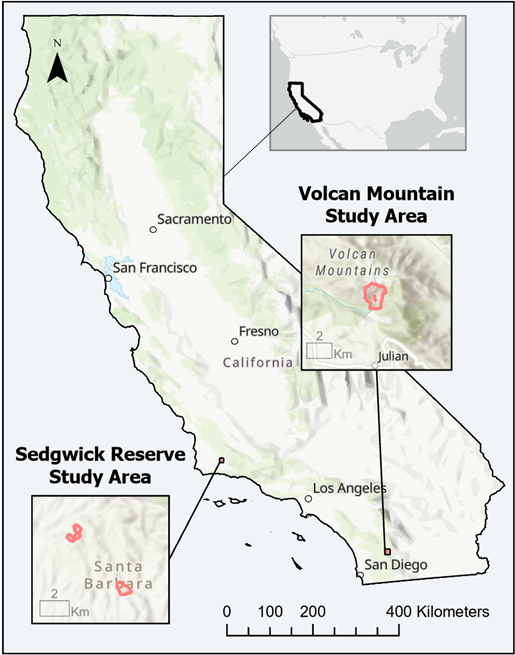
\includegraphics[trim=0mm 0mm 0mm 0mm, clip, width=\linewidth]
                  {manuscript/figures/Overall_Study_Areas_v2.png}
  \caption{Locations of the Southern California UAV LiDAR surveys—Sedgwick
           Reserve–Midland School in the Santa Ynez Valley and Volcan Mountain
           Wilderness Preserve in the Peninsular Range.}
  \label{fig:overall_study_area}
\end{wrapfigure}

The core challenge addressed by this research is the enhancement of sparse and outdated national airborne LiDAR datasets. To train and validate supervised upsampling models, we collected dense UAV LiDAR as a high-accuracy benchmark of actual vegetation structure. The sections below describe the study areas where this data was collected, the multi-modal input data sources, and steps taken to ensure spatial alignment and consistency across all modalities.

\subsection{Study Area}


The study area (Figure \ref{fig:overall_study_area}) consists of two separate sites in Southern California, USA.
The first study area includes parts of the 24-square-kilometer Sedgwick Reserve, managed by the University of California, Santa Barbara, and the adjacent 11.5 square kilometer Midland School property. Both sit within the San Rafael Mountain foothills of Santa Barbara County (Figure \ref{fig:sedgwick_study_area}). 


\begin{figure}
  \centering
  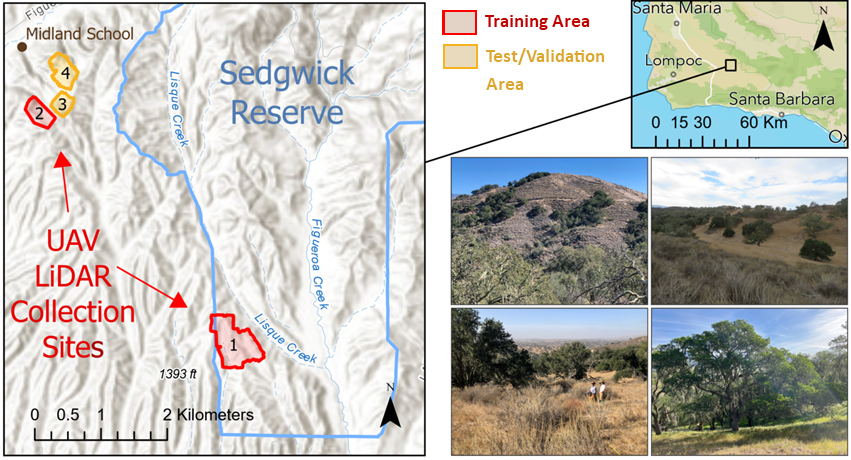
\includegraphics[width=1\linewidth]{manuscript/figures/Sedgwick_Reserve_Study_Area.png}
    \caption{The first study area combines parts of the Sedgwick Reserve and Midland School property in the San Rafael Mountain foothills, Santa Barbara County. It features diverse vegetation such as oak woodlands, chaparral, grasslands, and coastal sage scrub. Within this area, four UAV LiDAR sites were surveyed, covering a total of 70 hectares.}
  \label{fig:sedgwick_study_area}
\end{figure}
The area spans elevations from 287 to 852 meters and supports a diverse array of vegetation, including coastal sage scrub, native grasslands, chaparral, coast live and blue oak woodlands, valley oak savanna, riparian habitats, and gray pine forests. UAV LiDAR was collected on four sites (totaling about 71 hectares) within the study area (Table \ref{tab:lidar_sites}).


\vspace*{\fill} % push content down from above
\begin{table}[H] % 'H' forces exact placement
  \centering
  \caption{UAV LiDAR sites used as ground truth for model development}
  \label{tab:lidar_sites}
  \begin{tabular}{@{}cllll@{}}
    \toprule
    Site & Hectares & Location & Collection Date & Model Use\\ \midrule
    1 & 38 & Sedgwick Reserve & 30 Jun 2023 & Training\\
    2 & 11 & Midland School   & 23 Oct 2023 & Training\\
    3 & 12 & Midland School   & 23 Oct 2023 & Test/Validation\\
    4 & 9 & Midland School   & 28 Sep 2023 & Test/Validation\\
    5 & 197 & Volcan Mountain & 25 Oct 2024 & \begin{tabular}[c]{@{}l@{}}70\% Training\\ 30\% Test/Validation\end{tabular}\\
    \bottomrule
  \end{tabular}
\end{table}
\vspace*{\fill} % push content up from below
The second study area (Figure \ref{fig:volcan_mtn_study_area}) consists of 197 hectares within and adjacent to the Volcan Mountain Wilderness Preserve in the Peninsular Range of Southern California. The reserve is managed by San Diego County and the Volcan Mountain Foundation and ranges in elevation from about 1220 meters to over 1675 meters.
\newpage
 It hosts diverse plant communities, including oak woodlands, chaparral, mixed conifer forests, and grasslands.  To ensure robust model evaluation across this ecological gradient, roughly 30 percent of the area (58 hectares) was reserved for testing and validation (Table \ref{tab:lidar_sites}). The three holdout zones were selected to reflect the site’s vegetation diversity: the northernmost area includes chaparral that replaced forest following wildfires in 2003 and 2005; the central zone contains dense mixed-conifer and riparian vegetation interspersed with oak woodlands and chaparral; and the southernmost zone is predominantly semi-continuous oak canopy. 

\begin{figure}[!t]
    \centering
    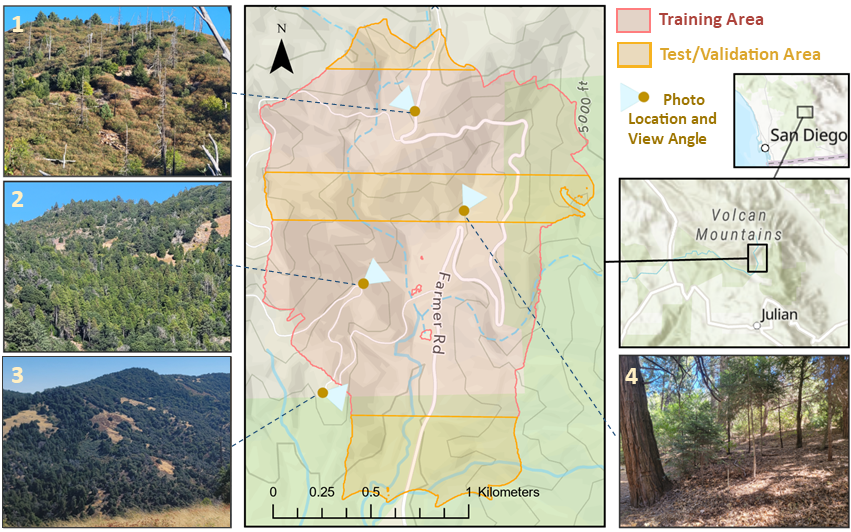
\includegraphics[width=1\linewidth]{manuscript/figures/Volcan_Mtn_Study_Area.png}
    \caption{Volcan Mountain study area (197 hectares) in the Peninsular Range of Southern California, encompassing diverse vegetation types across an elevation range of 1220 to 1675 meters. Thirty percent of the site (58 hectares) was set aside for testing/validation in three zones: post-fire chaparral in the north, mixed conifer and riparian vegetation with oak and chaparral in the center, and oak woodland with semi-continuous canopy in the south. }
    \label{fig:volcan_mtn_study_area}
\end{figure}






\subsection{The Data}

All remote‐sensing assets were co-registered within a common tiling framework covering both study sites.  
First, the UAV‐LiDAR acquisition footprints were tessellated into 10m × 10m analysis tiles with 15 \% overlap, yielding an \emph{initial} set of 9,800 tiles at Sedgwick–Midland and 26,557 tiles at Volcan Mountain.  Each tile served as the spatial key for assembling a four-layer data stack:

\begin{enumerate}[leftmargin=*]
    \item \textbf{UAV LiDAR} point clouds (\textit{Sedgwick}-2023, 300 pts/m\textsuperscript{2}; \textit{Volcan}–2024, 300 pts/m\textsuperscript{2})
    \item \textbf{3DEP airborne LiDAR} (\textit{Sedgwick}-2018, 22 pts/m\textsuperscript{2}; \textit{Volcan}-2015–16, 6 pts/m\textsuperscript{2})
    \item \textbf{UAVSAR radar} coverage from 2014 to 2024 (6.17 m GSD)
    \item \textbf{NAIP imagery} coverage from 2014 to 2022 (0.6–1 m GSD)
\end{enumerate}

By standardizing on overlapping 10 m patches, we guarantee that each training example draws from the same footprint across sensors—ensuring the model learns consistent, co-registered features from LiDAR, SAR, and imagery.

\subsubsection{UAV LiDAR Data}
\textit{Sedgwick and Midland Sites} - Between June and October 2023, UAV LiDAR data was collected by San Diego State Geography Department Staff on the Sedgwick and Midland School Sites using a DJI Matrice 300 drone equipped with a TrueView 515 LiDAR. The drone was flown at an altitude of approximately 60 meters above ground level, achieving a point density of around 300 points per square meter. 

\textit{Volcan Mountain Site} - On October 25, 2024, the same Geography Department staff conducted flights using a  DJI Matrice 350 drone equipped with a TrueView 540 LIDAR system. This newer drone and sensor was flown at a higher altitude of approximately 120 meters above ground level, and still achieved a point density of over 300 points per square meter.

\subsubsection{Crewed Airborne LiDAR}
The available crewed airborne LiDAR (C-ALS) data includes two separate 3DEP datasets. The  Sedgwick  3DEP dataset, collected in 2018, has a point density of 22 pts/m\textsuperscript{2}. The C-ALS data for the Volcan Mountain site was collected between October 2015 and November 2016 and has a point density of 6.3 pts/m\textsuperscript{2} \citep{usgs_usgs_2016}. Both datasets were  acquired via Microsoft's Planetary Computer \citep{us_geological_survey_3d_elevation_program_usgs_2023,planetary_computer}

\subsubsection{Synthetic Aperture Radar (SAR)}
Fully polarimetric L-band imagery (23.84 cm wavelength) from NASA’s UAVSAR system was acquired through the Alaska Satellite Facility’s \texttt{asf\_search} Python API \citep{alaska_search}.  The UAVSAR flights were conducted from a Gulfstream-III platform with bidirectional acquisitions from opposite look directions at an average altitude of 12,495 meters, providing multi-perspective radar coverage of the landscape at 6.17-meter ground resolution.

\begin{itemize}[leftmargin=1.5em]
  \item \textbf{Volcan Mountain}: Four campaigns —  June 11 2014 (3 looks), October 9 2014 (2), October 17 2018 (2), November 23 2021 (2) — all part of NASA’s San Andreas Fault monitoring program.
  \item \textbf{Sedgwick Reserve}: Four campaigns — June 23–24 2014 (8 looks), April 4 2016 (6), September 27–28 2023 (6), October 31 2024 (2) — the Sep 2023 campaign supported the \emph{NASA FireSense} initiative, while the others were routine San Andreas fault-monitoring acquisitions.
\end{itemize}


For every \SI{10}{m} × \SI{10}{m} 3DEP tile we extracted a co-centered \SI{20}{m} × \SI{20}{m} UAVSAR chip to accommodate layover and shadow extent, then bilinearly resampled each chip to \SI{5}{m} GSD before fusion with NAIP imagery and LiDAR. 



\subsubsection{High-Resolution Aerial Imagery}
We ingested NAIP imagery through the Microsoft Planetary Computer STAC API \citep{planetary_computer} for survey years 2014–2022.  
NAIP provides four-band (Red, Green, Blue, Near-Infrared) orthoimagery of the conterminous United States, collected at peak green-up on a two- to three-year cycle.  Prior to the 2016 flight season, data were delivered at 1 m ground-sample distance (GSD); since 2016 the native resolution has been 60 cm.

\begin{itemize}[leftmargin=1.5em]
  \item \textbf{Volcan Mountain}: May 2014 (1 m), Apr 2016 (60 cm), Aug 2018 (60 cm), Apr 2020 (60 cm), Apr 2022 (60 cm)
  \item \textbf{Sedgwick Reserve}: Jun 2014 (1 m), Jun 2016 (60 cm), Jul 2018 (60 cm), May 2020 (60 cm), May 2022 (60 cm)
\end{itemize}

For every 10 m × 10 m 3DEP tile we extracted a 20 m × 20 m NAIP chip centered on the same point to accommodate viewing-geometry variance and to capture neighboring shadows.  All NAIP scenes were then resampled to a common 50 cm grid.



\subsection{Data Cleaning and Preprocessing}
To reduce computational load and give the upsampling network a uniform-density target, we downsampled every tile with an adaptive anisotropic voxel grid. Each cloud was first voxelized at a 4 cm × 4 cm × 2 cm resolution; if more than 50 000 points remained, the horizontal voxel edge was incrementally enlarged (keeping the vertical edge at 50\% of that value) and the filter reapplied until the count fell below the limit. The resulting point sets preserve fine vertical structure while standardizing horizontal density. The dataset was partitioned into training, validation, and test sets using reference polygons to ensure the holdout sets captured the full environmental gradients found in the training data. We enforced quality constraints by requiring a UAV-to-3DEP point ratio above 2.0, and a minimum of 16000 UAV LiDAR points and 200 3DEP points per tile.


\subsection{Data Augmentation}
To improve model generalization across diverse terrain landscapes, we augmented our training data to expand it from 24,000 to 40,000 tiles. Our approach included a random assortment of point cloud-specific operations (random point removal, jittering) and standard geometric modifications (rotation and reflection) that were performed on the point cloud and imagery. We sampled the original training tiles without replacement , prioritizing those with high z-variance and large z-variance deviations from ground truth. 





\section{Methods}
Our multimodal upsampling framework transforms a sparse 3DEP point cloud, plus co-registered NAIP and UAVSAR image chips, into a denser 3-D point cloud (Fig.~\ref{fig:pipeline}).  
The network is built around the \textbf{Local–Global Point Attention Block} (LG-PAB; §\ref{sec:lgpab}), which provides permutation‐invariant feature learning, optional feature-guided upsampling, and long-range geometric context.  
Five macro–components are arranged in a feed-forward sequence:  
(1) point feature extraction, (2) imagery encoding, (3) cross-attention fusion, (4) feature expansion and refinement, and (5) point decoding.

\begin{figure}
    \vspace{-20pt}  
    \centering
    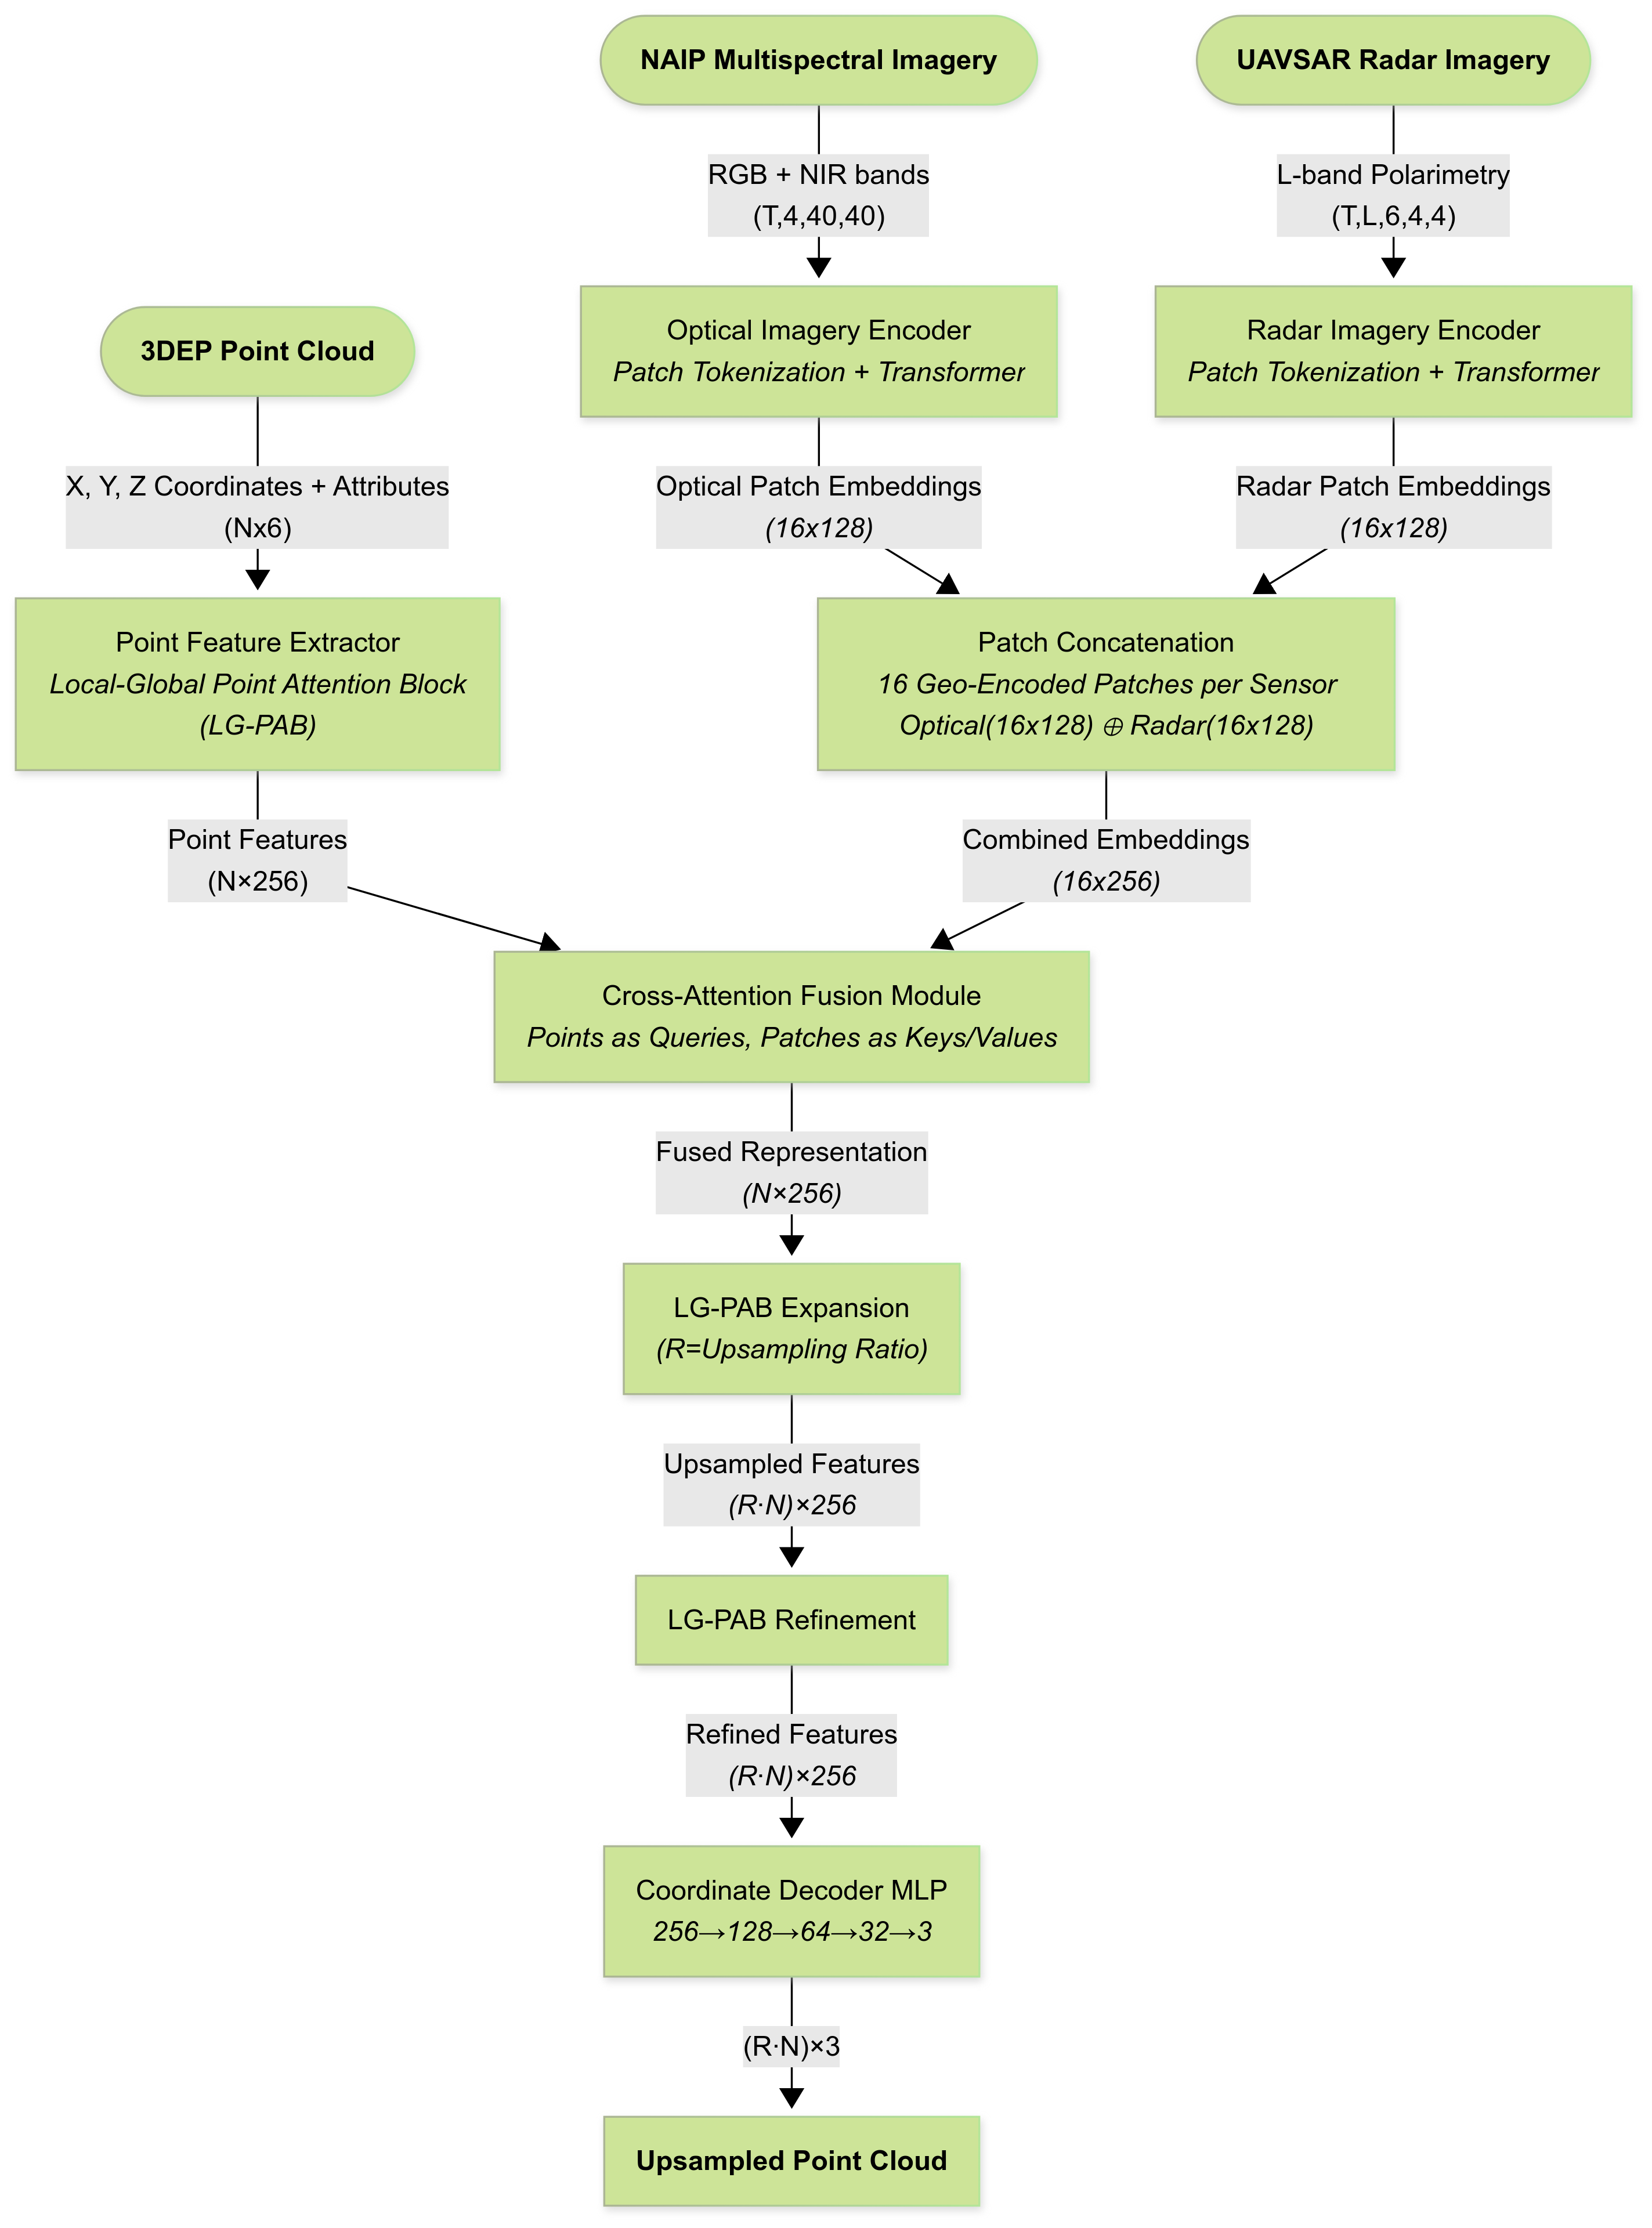
\includegraphics[trim=0mm 0mm 0mm 9mm, clip, width=1\linewidth]{manuscript/figures/Overall_Architecture.png}
    \caption{The overall multimodal upsampling architecture. Key components include Local–Global Point Attention Blocks, modality-specific imagery encoders for processing optical (NAIP) and radar (UAVSAR) data, and a cross-attention fusion module for combining imagery and LiDAR features.}
    \label{fig:pipeline}
\end{figure}


\subsection{Model Architecture}
\label{sec:architecture}

\paragraph{Notation Conventions.}
Throughout this section, we use the following notation for tensor dimensions:
\begin{itemize}
    \item Counts: $N_{\text{pts}}$ (number of input points), $N_{\text{curr\_pts}}$ (current points in LG-PAB), $N_{\text{pts\_up}} = R_{\text{up}} \cdot N_{\text{pts}}$ (upsampled points), $N_{\text{patch}}$ (number of image patches, default 16), $N_{\text{time}}$ (temporal stack length), $N_{\text{looks}}$ (maximum look angles, $\leq 2$).
    \item Dimensions: $D_{\text{coord}} = 3$ (coordinate dimension), $D_{\text{attr}}$ (attribute dimension), $D_{\text{p\_feat}} = 256$ (point feature dimension), $D_{\text{p\_in}}$ (input point feature dimension), $D_{\text{p\_out}}$ (output point feature dimension), $D_{\text{token}} = 128$ (token dimension).
    \item Channels: $C_{\text{naip}} = 4$ (NAIP channels), $C_{\text{uavsar}} = 6$ (UAVSAR channels).
    \item Image dimensions: $H_{\text{naip}} = W_{\text{naip}} = 40$ (NAIP height/width), $H_{\text{uavsar\_pr}} = W_{\text{uavsar\_pr}} = 4$ (UAVSAR patch region height/width).
    \item Other: $R_{\text{up}}$ (upsampling ratio, default 2), $k_{\text{knn}} = 16$ (k-nearest neighbors).
\end{itemize}
For tensors, we use the notation TensorSymbol: (dim$_1$, dim$_2$, ..., dim$_k$) to describe their dimensions.

Given an input cloud $P_{\text{in}}: (N_{\text{pts}}, D_{\text{coord}})$ with points $\{\mathbf{x}_i\}_{i=1}^{N_{\text{pts}}}\subset\mathbb{R}^{D_{\text{coord}}}$ and attributes $\mathbf{a}_i: (D_{\text{attr}})$, the network outputs $P_{\text{out}}: (N_{\text{pts\_up}}, D_{\text{coord}})$ with points $\{\hat{\mathbf{x}}_j\}_{j=1}^{N_{\text{pts\_up}}}$ where $N_{\text{pts\_up}} = R_{\text{up}} \cdot N_{\text{pts}}$ (typically $R_{\text{up}} = 2$).

An overview is:

\begin{enumerate}[leftmargin=*]
\item \textbf{LG-PAB Extractor} $\;\mathcal{E}_{\mathrm{pt}}$
      $\;\rightarrow$ local–global point features $F: (N_{\text{pts}}, D_{\text{p\_feat}})$;
\item \textbf{Imagery Encoders} $\;\mathcal{E}_{\mathrm{opt}},\mathcal{E}_{\mathrm{rad}}$
      $\;\rightarrow$ NAIP and UAVSAR patch embeddings $E_{\text{opt}}, E_{\text{rad}}: (N_{\text{patch}}, D_{\text{token}})$;
\item \textbf{Cross-Attention Fusion} $\;\mathcal{F}_{\mathrm{ca}}$
      $\;\rightarrow$ enriched point features $F_{\!\mathrm{fused}}: (N_{\text{pts}}, D_{\text{p\_feat}})$;
\item \textbf{LG-PAB Expansion \& Refinement}
      $\;\rightarrow$ upsampled features $F^{\uparrow}: (N_{\text{pts\_up}}, D_{\text{p\_feat}})$ and coordinates $P^{\uparrow}: (N_{\text{pts\_up}}, D_{\text{coord}})$;
\item \textbf{MLP Decoder} $\;\rightarrow$ residual offsets $\Delta P: (N_{\text{pts\_up}}, D_{\text{coord}})$ and final coordinates $P_{\mathrm{out}}: (N_{\text{pts\_up}}, D_{\text{coord}})$.
\end{enumerate}

% --- LG-PAB (its own page) ---------------------------------------------------
\clearpage
\subsection{The Local–Global Point Attention Block (LG-PAB)}
\label{sec:lgpab}

\begin{wrapfigure}[40]{r}{0.43\textwidth}
  \centering
  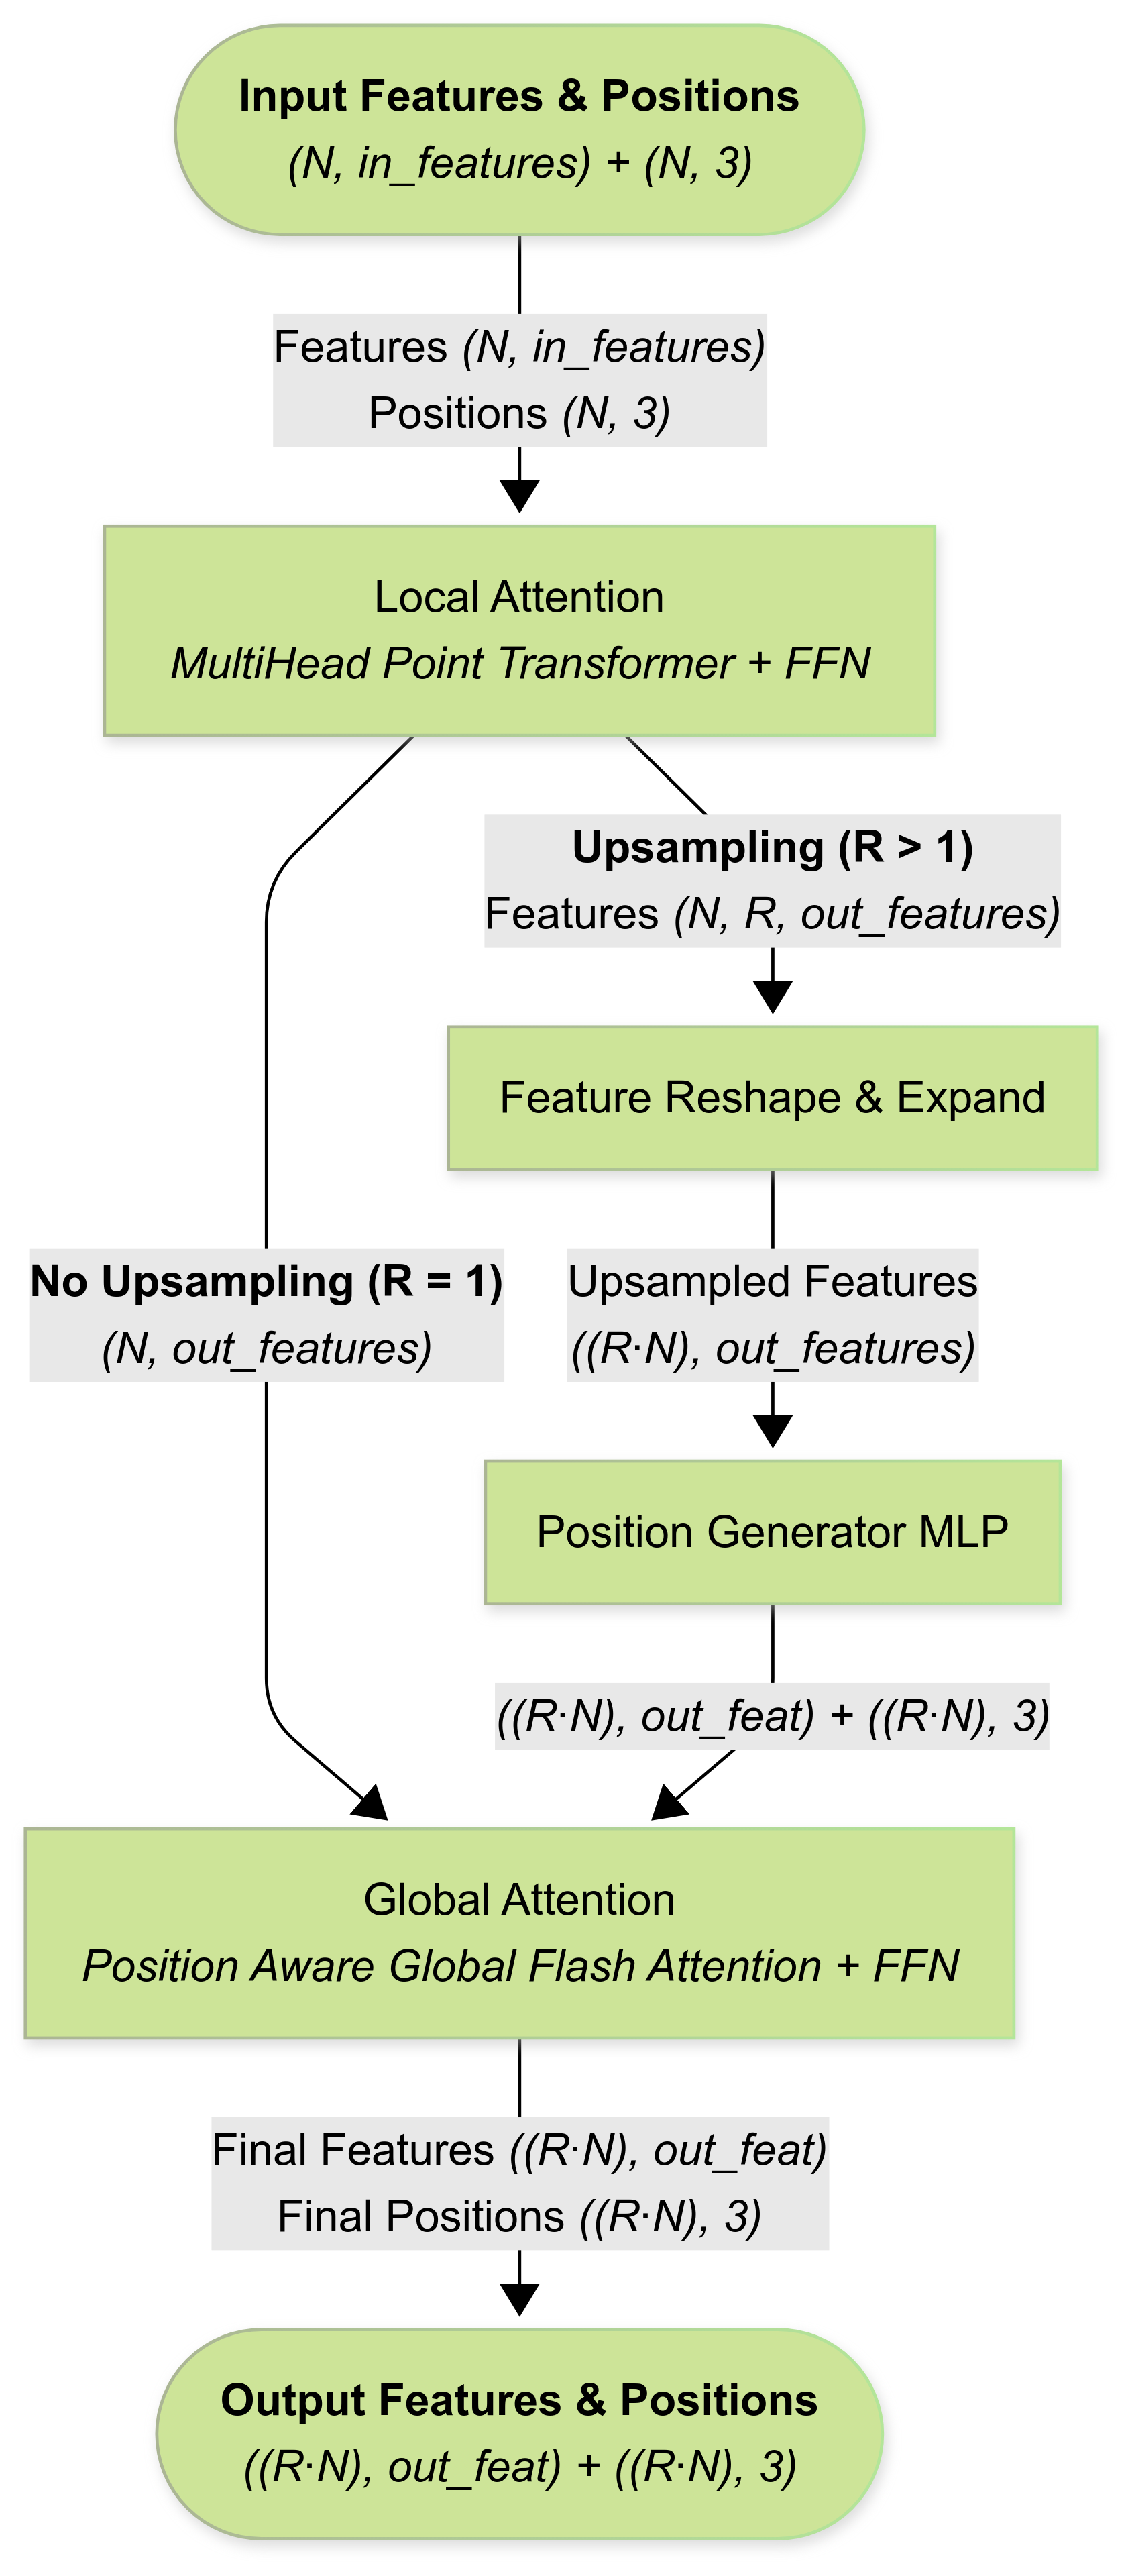
\includegraphics[trim=0mm 0mm 36mm 0mm, clip, width=0.43\textwidth]{manuscript/figures/LG-PAB.png}
  \caption{Flowchart of the Local–Global Point Attention Block (LG-PAB), the core computational unit used across the feature extraction, expansion, and refinement stages. The block applies local attention via a multi-head Point Transformer, optional upsampling with learned position offsets, and global multi-head Flash Attention for broader spatial context. A feed-forward MLP follows both the local and global attention blocks.} 
  \label{fig:lgpab}
\end{wrapfigure}%

Figure~\ref{fig:lgpab} presents a flow-chart of the \emph{Local–Global Point Attention Block}, the fundamental unit used three times in our architecture (extraction, expansion, and refinement stages).  
Each LG-PAB converts an input tuple $\langle X, P \rangle$ consisting of point features $X: (N_{\text{curr\_pts}}, D_{\text{p\_in}})$ and 3-D coordinates $P: (N_{\text{curr\_pts}}, D_{\text{coord}})$ into refined (and optionally upsampled) features and positions. The block proceeds through the stages that appear in the diagram:

\begin{enumerate}[leftmargin=*]
\item \textbf{Local Attention Block}  
      A \textsc{Multi-Head Point Transformer} operates on a $k_{\text{knn}}$-nearest-neighbour graph ($k_{\text{knn}}{=}16$) to capture fine-scale geometry. Its output passes through a two-layer \textsc{Feed-Forward Network} (FFN) with GELU activation, producing an intermediate tensor 
      $Z: (N_{\text{curr\_pts}}, R_{\text{up}} \cdot D_{\text{p\_out}})$.  
      When the upsampling ratio $R_{\text{up}}{=}1$ this step already delivers the final per-point features.

\item[\emph{2\,a}] \textbf{Feature-Guided Upsampling (optional)}  
      If $R_{\text{up}}{>}1$ (expansion stage) the intermediate tensor is reshaped to $[N_{\text{curr\_pts}}, R_{\text{up}}, D_{\text{p\_out}}]$, effectively cloning each feature vector $R_{\text{up}}$ times.  
      A small \textbf{Position-Generator MLP} then predicts a 3-D offset for every clone, yielding new coordinates  
      $\hat{P} = P^{\text{rep}} + \Delta P: (N_{\text{curr\_pts}} \cdot R_{\text{up}}, D_{\text{coord}})$.  
      The features are flattened back to $[N_{\text{curr\_pts}} \cdot R_{\text{up}}, D_{\text{p\_out}}]$.

\item \textbf{Global Attention Block}  
      To impose long-range coherence, the upsampled (or original) features are processed by \textsc{Position-Aware Global Flash Attention}. Coordinates are first embedded by a two-layer MLP, concatenated to the features, and fed to a four-head FlashAttention layer that attends across \emph{all} points in the tile. A second FFN refines the attended features, after which residual connections and LayerNorm complete the block.
\end{enumerate}

% --- Imagery Encoders (its own page) ----------------------------------------
\clearpage
\subsection{Imagery Encoders}
\label{sec:img_enc}

\begin{wrapfigure}[20]{r}{0.45\textwidth}
  \vspace{-25pt}  
  \centering
  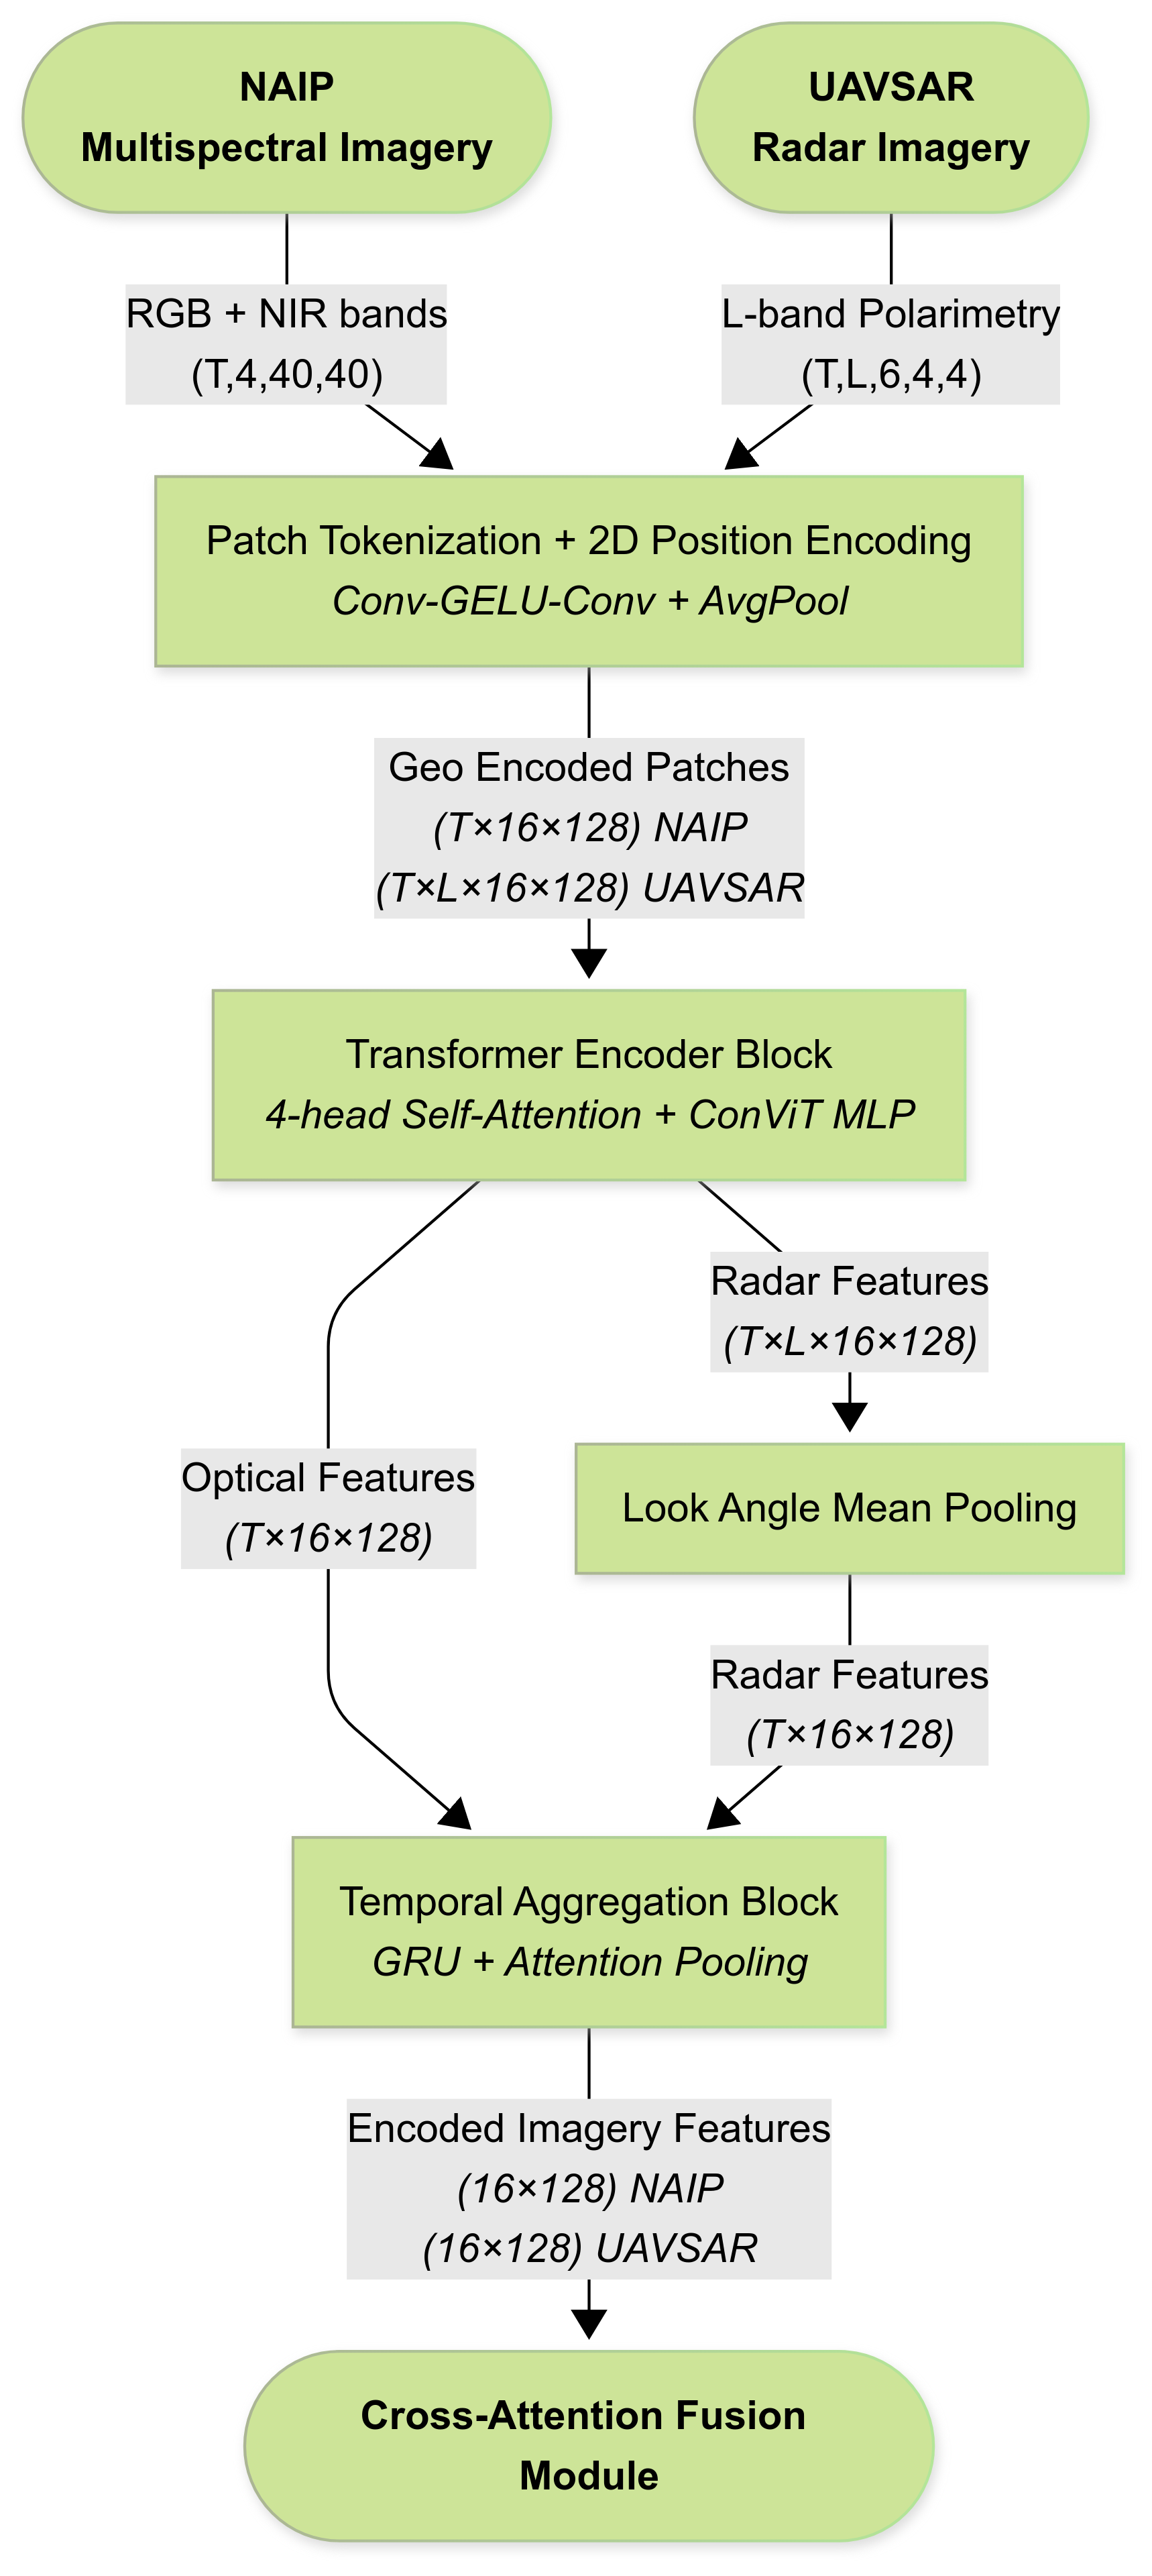
\includegraphics[trim=0mm 0mm 20mm 0mm, clip, width=0.43\textwidth]{manuscript/figures/Imagery_Encoders.png}
  \caption{Architecture diagram of the imagery encoders. Image stacks from NAIP (optical) and UAVSAR (radar) pass sequentially through Patch Tokenization, Transformer Encoder blocks for spatial context modeling, and a Temporal GRU-Attention Head for temporal aggregation.}
  \label{fig:imgenc}
\end{wrapfigure}%

Optical (NAIP) and radar (UAVSAR) image chips are processed by a \emph{shared five-stage encoder} (with modality specific weights) that converts each image stack into a fixed set of patch tokens. The encoder stages—illustrated in Fig.~\ref{fig:imgenc}—are:

\begin{enumerate}[leftmargin=*]      
\item \textbf{Patch Tokenization.}  
      A two-layer Conv–GELU–Conv stem with stride-1 followed by average pooling (stride=$\texttt{patch\_size}$) extracts features on a $4\times4$ grid.  
      This design mirrors Shifted Patch Tokenization, which adds local texture bias to ViTs and improves sample efficiency on small datasets \citep{lee2021vision}.  
      The $N_{\text{patch}}=16$ patches are flattened to $Z_{\text{tok}}: (N_{\text{patch}}, D_{\text{token}})$ and normalized via LayerNorm.


\item \textbf{2-D Positional Encoding.}  
      Normalized patch centers are embedded via a two-layer MLP and added to the tokens:  
      $Z_{\text{pos}} = Z_{\text{tok}} + \text{MLP}_{\text{pos}}(x,y)$.

\item \textbf{Transformer Encoder Block.}  
      A 4-head self-attention layer is paired with LayerScale ($\gamma \approx 10^{-5}$), a learnable scalar that stabilizes deep transformers \citep{touvron2021going}.  
      The accompanying MLP includes a depth-wise 1-D convolution, following the ConViT approach to introduce a soft convolutional inductive bias \citep{dascoli2021convit}.  
      The block outputs $Z_{\text{enc}}: (N_{\text{patch}}, D_{\text{token}})$.


\item \textbf{Temporal GRU–Attention Head.}  
      For inputs with temporal length $N_{\text{time}}$, a bidirectional GRU with attention pooling aggregates tokens into patch descriptors $E_{\text{patch}}: (N_{\text{patch}}, D_{\text{token}})$.
\end{enumerate}

\paragraph{UAVSAR Look Angle Mean Pooling}
\begin{itemize}[leftmargin=*]
\item \textbf{UAVSAR.}  
      Input $I_{\text{uavsar}}: (N_{\text{time}}, N_{\text{looks}}, C_{\text{uavsar}}, H_{\text{uavsar\_pr}}, W_{\text{uavsar\_pr}})$ with $N_{\text{looks}} \leq 2$.  
      After stage 3, we average features across available look angles to produce $Z_{\text{avg}}: (N_{\text{time}}, N_{\text{patch}}, D_{\text{token}})$ before temporal processing.
      Otherwise, the pipeline matches NAIP.
\end{itemize}


Both encoders output token matrices $E_{\text{opt}}$ and $E_{\text{rad}}: (N_{\text{patch}}, D_{\text{token}})$ that are normalized and concatenated before fusion.



\clearpage

\subsection{End-to-End Upsampling Pipeline}
\label{sec:pipeline}

\paragraph{1) Local–Global Feature Extraction.}
The sparse 3DEP cloud—concatenated with intensity, return number, and number or returns (6 attributes total)—is processed by the first \emph{Local–Global Point Attention Block} (§\ref{sec:lgpab}). The output is a set of point features $F: (N_{\text{pts}}, D_{\text{p\_feat}})$ that encode both neighborhood morphology and tile-level context.

\paragraph{2) Imagery Encoders.}
Co-registered NAIP and UAVSAR chips are independently tokenized and fed to lightweight Transformer encoders ($N_{\text{patch}}$ patches, embed dim $D_{\text{token}}$).  
The optical encoder (\textcolor{blue}{RGB+NIR}) outputs patch embeddings $E_{\text{opt}}: (N_{\text{patch}}, D_{\text{token}})$, whereas the radar encoder (\textcolor{blue}{L-band polarimetry}) outputs $E_{\text{rad}}: (N_{\text{patch}}, D_{\text{token}})$.  
When multiple acquisition dates exist, per-modality tokens are fused temporally via a shared GRU–attention head.

\paragraph{3) Cross-Attention Fusion.}
Point features act as \emph{queries} and image patches as \emph{keys/values} in a four-head cross-attention block.  
Scaled dot-product scores are masked for patches whose centroid is more than 8 meters from the query point. 
The fused representation $F_{\text{fused}}: (N_{\text{pts}}, D_{\text{p\_feat}})$ augments every point with spectral texture and volumetric back-scatter cues, improving discrimination of canopy surfaces versus gaps.

\paragraph{4) Feature-Guided Upsampling.}
A second LG-PAB with ratio $R_{\text{up}}=2$ expands $F_{\text{fused}}$ and predicts offsets $\Delta P$ that generate $N_{\text{pts\_up}}$ candidate coordinates. This stage doubles point density while maintaining local topology.

\paragraph{5) Feature Refinement.}
A third LG-PAB (ratio $R_{\text{up}}=1$) re-computes local and global attention on the enlarged cloud, ironing out artifacts introduced during expansion and propagating context across newly formed neighborhoods.

\paragraph{6) Coordinate Decoding.}
Finally, a four-layer MLP ($D_{\text{p\_feat}} \rightarrow 128 \rightarrow 64 \rightarrow 32 \rightarrow D_{\text{coord}}$) regresses residual offsets that are added to the upsampled positions, producing the higher-resolution prediction $\hat{P}: (N_{\text{pts\_up}}, D_{\text{coord}})$.

%-------------------------------------------------
\subsection{Training Protocol}
\label{sec:study_design}
%-------------------------------------------------

%---------------------------------------------------------------
% 1) Dataset preparation
%---------------------------------------------------------------
\begin{table}[htbp]
  \centering
  \caption{Dataset preparation}
  \label{tab:data_prep}
  \begin{tabular}{lr}
    \toprule
    \textbf{Subset} & \textbf{Tiles} \\
    \midrule
    Training        & 24\,000 original $+$ 16\,000 augmented $=$ 40\,000 \\
    Validation      & 3\,792 \\
    Test            & 5\,688 \\
    \bottomrule
  \end{tabular}
\end{table}

%---------------------------------------------------------------
% 2) Model variants
%---------------------------------------------------------------
\begin{table}[htbp]
  \centering
  \caption{Model variants evaluated}
  \label{tab:model_variants}
  \begin{tabular}{lll}
    \toprule
    \textbf{Variant} & \textbf{Active encoders} & \textbf{Cross-attention on} \\
    \midrule
    Baseline   & LiDAR only                    & None \\
    + NAIP     & LiDAR, optical                & NAIP tokens \\
    + UAVSAR   & LiDAR, radar                  & UAVSAR tokens \\
    Fused      & LiDAR, optical, radar         & Concatenated tokens \\
    \bottomrule
  \end{tabular}
\end{table}

\begin{table}[htbp]
  \centering
  \caption{Model-configuration parameters}
  \label{tab:model_config_a}
  %          col 1            col 2             col 3 (wraps)
  \begin{tabular}{l c p{0.55\linewidth}}
    \toprule
    \textbf{Parameter} & \textbf{Value} & \textbf{Notes} \\
    \midrule
    \multicolumn{2}{c}{\textit{Core geometry}} \\
    Point-feature dimension        & 256 & — \\
    KNN neighbours ($k$)           & 16  & Used in local attention graph \\
    Upsampling ratio ($R_{\text{up}}$) & 2 & Doubles point density per LG-PAB expansion \\
    Point-attention dropout        & 0.02 & Dropout inside global attention heads \\
    \addlinespace
    \multicolumn{2}{c}{\textit{Attention-head counts}} \\
    Extractor — local / global     & 8 / 4 & Extra local heads help expand feature set \\
    Expansion — local / global     & 8 / 4 & Extra local heads aid point upsampling \\
    Refinement — local / global    & 4 / 4 & — \\
    \addlinespace
    \multicolumn{2}{c}{\textit{Imagery encoders}} \\
    Image-token dimension          & 128 & Patch embeddings for NAIP \& UAVSAR encoders \\
    \addlinespace
    \multicolumn{2}{c}{\textit{Cross-modality fusion}} \\
    Fusion heads                   & 4   & — \\
    Fusion dropout                 & 0.02 & — \\
    Positional-encoding dimension  & 36  & — \\
    \bottomrule
  \end{tabular}
\end{table}


%---------------------------------------------------------------
% 3) Training protocol and hardware
%---------------------------------------------------------------
\begin{table}[htbp]
  \centering
  \caption{Training protocol and hardware}
  \label{tab:training_protocol}
  \begin{tabular}{lp{0.62\linewidth}}
    \toprule
    \textbf{Setting} & \textbf{Value} \\
    \midrule
    Hardware      & 4\,×\,NVIDIA L40 (48 GB) GPUs under PyTorch DDP \\
    Optimizer     & \textit{ScheduleFreeAdamW} \citep{defazio_road_2024}; base LR $5\times10^{-4}$, weight-decay $10^{-4}$, $\beta_{1,2}=(0.9,0.999)$; no external LR schedule \\
    Loss function & Density-aware Chamfer distance (Eq. 9 in \citep{wu_density-aware_2021}), $\alpha=4$ \\
    Batch size    & 15 tiles per GPU \\
    Epochs        & 100 \\
    Gradient clip & $\lVert g\rVert_2 \le 10$ \\
    Training time & ≈ 7 h per model variant \\
    Model selection & Epoch with lowest validation loss \\
    \bottomrule
  \end{tabular}
\end{table}
\FloatBarrier   



\section*{Results}

We evaluated our research questions using non-parametric statistical tests to account for non-normality in the error distribution. For RQ1 and RQ2, we used Wilcoxon signed-rank tests to compare reconstruction error (measured by Chamfer distance) between models, with median percentage change and rank-biserial correlation as effect size measures. For RQ3, we used Spearman rank correlations to analyze the relationship between reconstruction error and absolute canopy height change across all models. We further split the dataset into canopy gains (N=2423) and losses (N=3264) to examine potential asymmetries in error patterns. Fisher r-to-z transformations were used to statistically compare correlation coefficients between models. All significance values are reported at $\alpha$=0.05, with bold values indicating statistically significant results.

\begin{table}[htbp]
\centering
\caption{Descriptive Statistics for Chamfer Distance Across All Models}
\begin{tabular}{lcccc}
\toprule
\textbf{Model} & \textbf{Mean CD (m)} & \textbf{Median CD (m)} & \textbf{Std Dev (m)} & \textbf{IQR (m)} \\
\midrule
Input & 2.568 & 0.858 & 6.852 & 1.540 \\
Baseline & 1.043 & 0.340 & 5.717 & 0.465 \\
NAIP & 0.993 & 0.316 & 5.542 & 0.421 \\
UAVSAR & 0.924 & 0.331 & 5.505 & 0.437 \\
Fused & 0.965 & 0.298 & 5.753 & 0.393 \\
\bottomrule
\end{tabular}
\label{tab:descriptive_stats}
\end{table}


\begin{table}[htbp]
\centering
\caption{RQ1: Effect of Individual Modalities on Reconstruction Error}
\begin{tabular}{lcc}
\toprule
\textbf{Comparison} & \textbf{Median Change (\%)} & \textbf{Effect Size} \\
\midrule
NAIP vs Baseline & \textbf{0.5} (p$<$0.001) & \textbf{0.088} \\
UAVSAR vs Baseline & \textbf{0.3} (p$<$0.001) & \textbf{0.062} \\
\bottomrule
\end{tabular}
\label{tab:rq1_results}
\end{table}
Both high-resolution optical imagery (NAIP) and L-band SAR imagery significantly reduced reconstruction error compared to the LiDAR-only baseline, with optical imagery providing slightly larger improvements (0.5\% vs 0.3\%). While statistically significant, the modest effect sizes (0.088 and 0.062 respectively) suggests that single-modality improvements over the baseline upsampling approach are limited in magnitude or may be concentrated in a limited number of tiles.

\begin{table}[htbp]
\centering
\caption{RQ2: Effect of Fusing Multiple Modalities on Reconstruction Error}
\begin{tabular}{lcc}
\toprule
\textbf{Comparison} & \textbf{Median Change (\%)} & \textbf{Effect Size} \\
\midrule
Fused vs NAIP & \textbf{0.7} (p$<$0.001) & \textbf{0.133} \\
\bottomrule
\end{tabular}
\label{tab:rq2_results}
\end{table}

The fusion of both optical and SAR imagery yielded additional reconstruction accuracy gains (0.7\% median reduction) beyond using NAIP alone, with a stronger effect size (0.133) than either individual modality achieved in RQ1. This statistically significant improvement supports our hypothesis that the two modalities contain complementary information that can be effectively combined through attention-based fusion. The results demonstrate that multi-modality approaches can leverage different sensing capabilities to achieve superior point cloud reconstruction.

\begin{table}[htbp]
\centering
\caption{RQ3: Correlation Between Reconstruction Error and Canopy Height Change}
\begin{tabular}{lcc}
\toprule
\textbf{Model} & \textbf{Spearman ρ} & \textbf{p-value} \\
\midrule
Baseline & \textbf{0.650} & p$<$0.001 \\
NAIP & \textbf{0.612} & p$<$0.001 \\
UAVSAR & \textbf{0.628} & p$<$0.001 \\
Fused & \textbf{0.582} & p$<$0.001 \\
\midrule
Baseline vs NAIP (z) & \textbf{3.377} & p$<$0.001 \\
Baseline vs UAVSAR (z) & \textbf{1.999} & p=0.046 \\
Baseline vs Fused (z) & \textbf{5.868} & p$<$0.001 \\
\bottomrule
\end{tabular}
\label{tab:rq3_results}
\end{table}


\begin{table}[htbp]
\centering
\caption{RQ3 Extended: Correlation Between Reconstruction Error and Canopy Height Changes (Gains vs. Losses)}
\begin{tabular}{lcccc}
\toprule
\multirow{2}{*}{\textbf{Model}} & \multicolumn{2}{c}{\textbf{Canopy Gains (N=2423)}} & \multicolumn{2}{c}{\textbf{Canopy Losses (N=3264)}} \\
\cmidrule(lr){2-3} \cmidrule(lr){4-5}
 & \textbf{Spearman ρ} & \textbf{p-value} & \textbf{Spearman ρ} & \textbf{p-value} \\
\midrule
Baseline & \textbf{0.601} & p$<$0.001 & \textbf{0.671} & p$<$0.001 \\
Naip & \textbf{0.586} & p$<$0.001 & \textbf{0.621} & p$<$0.001 \\
Uavsar & \textbf{0.597} & p$<$0.001 & \textbf{0.637} & p$<$0.001 \\
Fused & \textbf{0.587} & p$<$0.001 & \textbf{0.580} & p$<$0.001 \\
\midrule
Baseline vs Naip (z) & 0.825 & p=0.409 & \textbf{3.440} & p$<$0.001 \\
Baseline vs Uavsar (z) & 0.233 & p=0.816 & \textbf{2.406} & p=0.016 \\
Baseline vs Fused (z) & 0.768 & p=0.442 & \textbf{6.074} & p$<$0.001 \\
\bottomrule
\end{tabular}
\label{tab:rq3_extended_results}
\end{table}


All models showed strong correlations with absolute canopy height change, confirming that reconstruction error systematically increases with vegetation structure changes since the original LiDAR collection. The baseline model exhibited the strongest correlation with canopy change ($\rho=0.650$), while the fused model showed the weakest ($\rho=0.582$), with this difference being statistically significant ($z=5.868$, $p<0.001$). Importantly, the extended analysis revealed this pattern was driven primarily by canopy losses, where the baseline model performed significantly worse than all other models, particularly the fusion approach ($z=6.074$, $p<0.001$), while for canopy gains, all models performed similarly without statistically significant differences. These findings partially support our hypothesis that advanced models better mitigate error from canopy changes, but specifically for canopy removal scenarios where legacy LiDAR contains no information about the removed vegetation.

\section{Discussion}

\begin{figure}
    \centering
    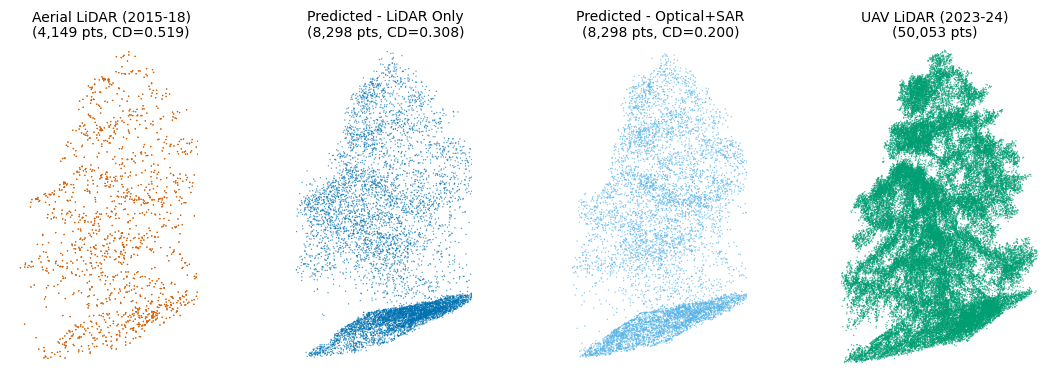
\includegraphics[width=1\linewidth]{manuscript/figures/model_output_example.png}
    \caption{Example tile where no major vegetation change occurred between the 3DEP aerial LiDAR (2015--2018) and UAV LiDAR (2023--2024). The optical+SAR fusion model more accurately recovers fine-scale canopy structure compared to the LiDAR-only model, producing a point cloud that more closely matches the UAV LiDAR reference (lower Chamfer Distance).}
    \label{fig:enter-label}
\end{figure}

\begin{figure}
    \centering
    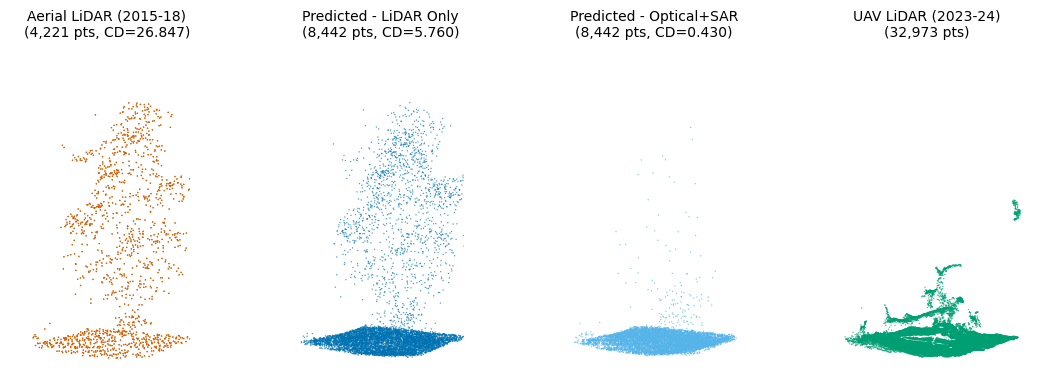
\includegraphics[width=1\linewidth]{manuscript/figures/canopy_loss_prediction.png}
    \caption{Example tile illustrating vegetation structure change between legacy aerial LiDAR (2015--2018) and recent UAV LiDAR (2023--2024). The optical+SAR fusion model accurately reconstructs the canopy loss visible in the UAV LiDAR reference, whereas the LiDAR-only model retains outdated structure from the earlier survey. This highlights the value of multi-modal imagery in correcting legacy LiDAR and detecting structural change.}
    \label{fig:enter-label}
\end{figure}

This study demonstrates the significant potential of attention-based deep learning models to enhance sparse and outdated airborne LiDAR point clouds by fusing them with more frequently acquired optical (NAIP) and Synthetic Aperture Radar (UAVSAR) imagery. Our findings directly address the critical need for up-to-date, high-resolution 3D vegetation structure information in applications like wildfire risk modeling and ecological monitoring.

The core success of our approach lies in the effective fusion of multi-modal data. As hypothesized (RQ1), both NAIP optical imagery and L-band UAVSAR imagery, when individually integrated, improved point cloud reconstruction accuracy compared to a baseline model relying solely on sparse LiDAR. NAIP, with its finer spatial resolution, offered a slightly greater enhancement, likely due to its ability to delineate canopy edges and small gaps with high fidelity. However, the true advancement was observed when these modalities were combined (RQ2). The fused model, leveraging both NAIP's textural detail and UAVSAR's structural sensitivity, outperformed single-modality enhancements. This confirms our hypothesis that these sensors provide complementary, rather than redundant, information, and that the cross-attention mechanisms within our architecture can effectively identify and leverage these synergistic relationships. This synergy is particularly valuable for capturing the complex, heterogeneous nature of vegetation.

Our investigation into temporal dynamics (RQ3) revealed that all models, including the baseline, exhibited increased reconstruction error in areas with substantial canopy change since the initial LiDAR survey. This is expected, as the input LiDAR reflects a past state. However, the fused model demonstrated the most robust performance, showing a significantly weaker correlation between error and the magnitude of canopy change, especially in areas of canopy loss. This is a crucial finding: by incorporating contemporaneous imagery, particularly the optical data that clearly depicts vegetation absence, the model can more effectively correct for outdated LiDAR information. The baseline model, lacking this current-state information, struggled most in loss scenarios. Even in areas of canopy growth, while not as pronounced as with loss, the image-informed models offered an advantage by providing cues about new or denser vegetation that the original sparse LiDAR could not capture. This capacity to "update" historical LiDAR datasets significantly enhances their utility for long-term monitoring and management, especially in landscapes prone to rapid changes from disturbances or growth.

The developed Local-Global Point Attention Block (LG-PAB) proved to be a robust architectural component. Its ability to capture both fine-grained local details through neighborhood-level self-attention and broader structural coherence via global attention across the entire point patch is central to its success. This hierarchical attention is well-suited to the fractal-like patterns often observed in natural vegetation.

Despite these promising results, some limitations exist. The improvements, while statistically significant, were modest in terms of percentage change in Chamfer distance. This suggests that while fusion helps, there might be inherent limits to upsampling very sparse LiDAR or that the current metrics may not fully capture all aspects of structural improvement relevant to ecological applications. Furthermore, our study was conducted in Southern California's Mediterranean ecosystems; model performance and the relative contributions of optical versus radar data might vary in different biomes with distinct vegetation structures and phenology.

A recommended area for future research involves adapting the validated multi-modal feature extraction pipeline for direct prediction of key vegetation structure rasters, such as Canopy Height Models (CHM), canopy cover, Above-Ground Biomass (AGB), and fuel types. Such an adaptation would entail replacing the current point cloud generation head with task-specific regression or classification heads, potentially broadening the practical applicability of this work. Integrating geometric priors, like Digital Surface Models (DSMs) and Digital Terrain Models (DTMs), into the loss function also represents a valuable direction. This could not only enforce greater structural realism but also enable the calculation of reconstruction error at various canopy strata, offering deeper insights into model performance. Furthermore, fine-tuning emerging foundation-model vision transformers, such as the Clay model, as shared encoders for NAIP and UAVSAR imagery, warrants exploration to leverage large-scale pretraining for enhanced feature representation. Complementary investigations could include a thorough evaluation of the UAVSAR encoder, particularly optimizing multi-look fusion beyond simple averaging and assessing resampling impacts, alongside ablation studies on the LG-PAB and imagery encoders to pinpoint key architectural contributions and guide further optimization.


\section{Conclusion}

This research successfully demonstrates that attention-based deep learning, leveraging our novel Local-Global Point Attention Block, can significantly enhance sparse airborne LiDAR point clouds in natural landscapes through the fusion of contemporaneous optical and radar imagery. We have shown that while individual imagery modalities provide benefits, their combined use yields superior reconstruction accuracy, particularly in mitigating errors arising from vegetation changes over time. Specifically, high-resolution optical imagery (NAIP) proved slightly more effective as a standalone ancillary dataset than L-band SAR within our framework, but the fusion of both offered the best performance, validating the complementary nature of these sensors. A key contribution is the model's ability to substantially reduce reconstruction degradation in areas of vegetation loss, thereby increasing the utility of historical LiDAR archives. This study presents a novel approach to direct 3D point cloud upsampling using multi-modal fusion in complex natural environments, moving beyond prevalent raster-based enhancement techniques and paving the way for more accurate and timely assessments of vegetation structure.






\section*{References}

\bibliography{manuscript/references}



\section{Appendix}


\begin{figure}
    \centering
    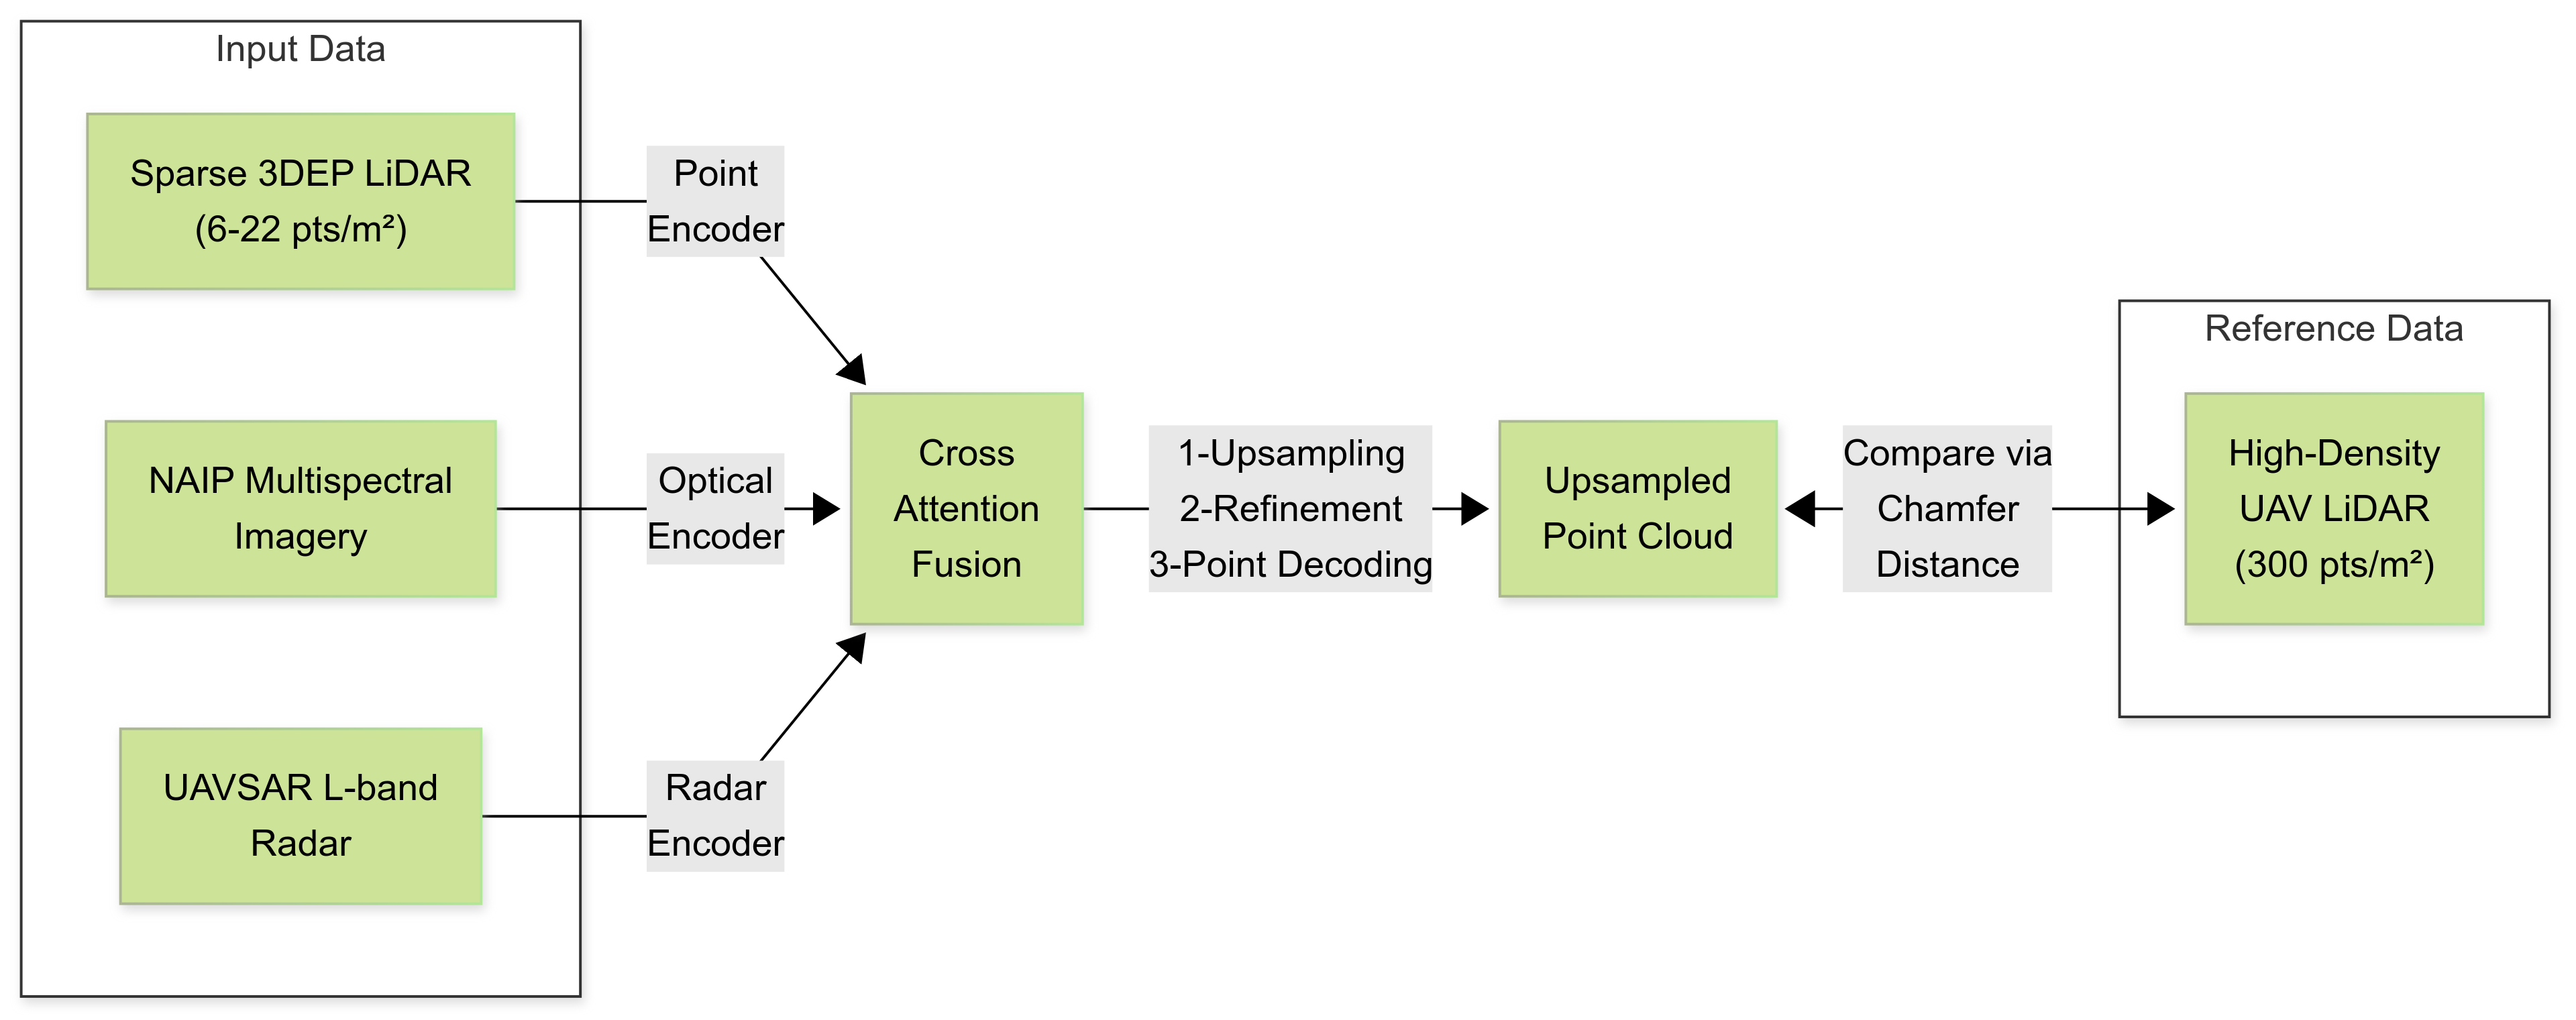
\includegraphics[width=\linewidth]{manuscript/figures/high_level_overview.png}
    \caption{High level workflow overview}
    \label{fig:enter-label}
\end{figure}
\end{document}
